\begin{figure}[htbp]
    \centering
    \subfloat[Model 0.]{
        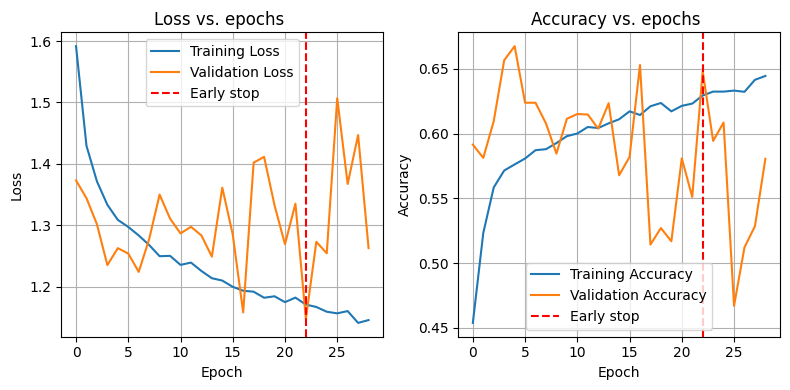
\includegraphics[width=0.7\textwidth]{figures/images/epochs_m0.png}
        \label{fig:epochs_m0}
    }
    \\
    \subfloat[Model 1.]{
        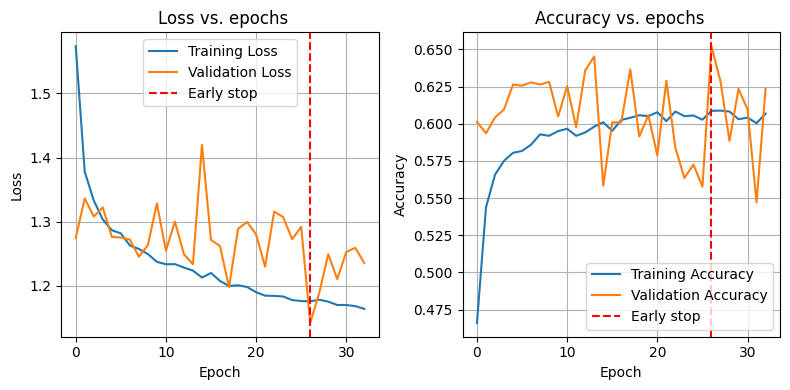
\includegraphics[width=0.7\textwidth]{figures/images/epochs_m1.png}
        \label{fig:epochs_m1}
    }
    \caption{Graph of loss and accuracy of the two models during the training phase, highlighting the point of early stopping.}
    \label{fig:epochs}
\end{figure}